% Chapter 5 - System Description

\chapter{System Description}
\label{Chapter5}

%----------------------------------------------------------------------------------------

This chapter describes the system implementation and demonstrates how users interact with the platform. The chapter begins by showing the visualizations inherited from TECVis 1.0, then presents the new features and enhancements in TECVis 2.0.

%----------------------------------------------------------------------------------------

\section{TECVis 1.0 Visualizations}

TECVis 1.0 provided two core visualizations that enabled geographic and temporal comparison of emotions. These visualizations are preserved in TECVis 2.0, benefiting from improved emotion detection accuracy while maintaining the same user experience.

\subsection{Dot Plot Visualization}

The dot plot visualization, inherited from TECVis 1.0, displays emotion scores across all US states. Figure~\ref{fig:landing_page} shows the main dashboard with this visualization.

\begin{figure}[htbp]
\centering
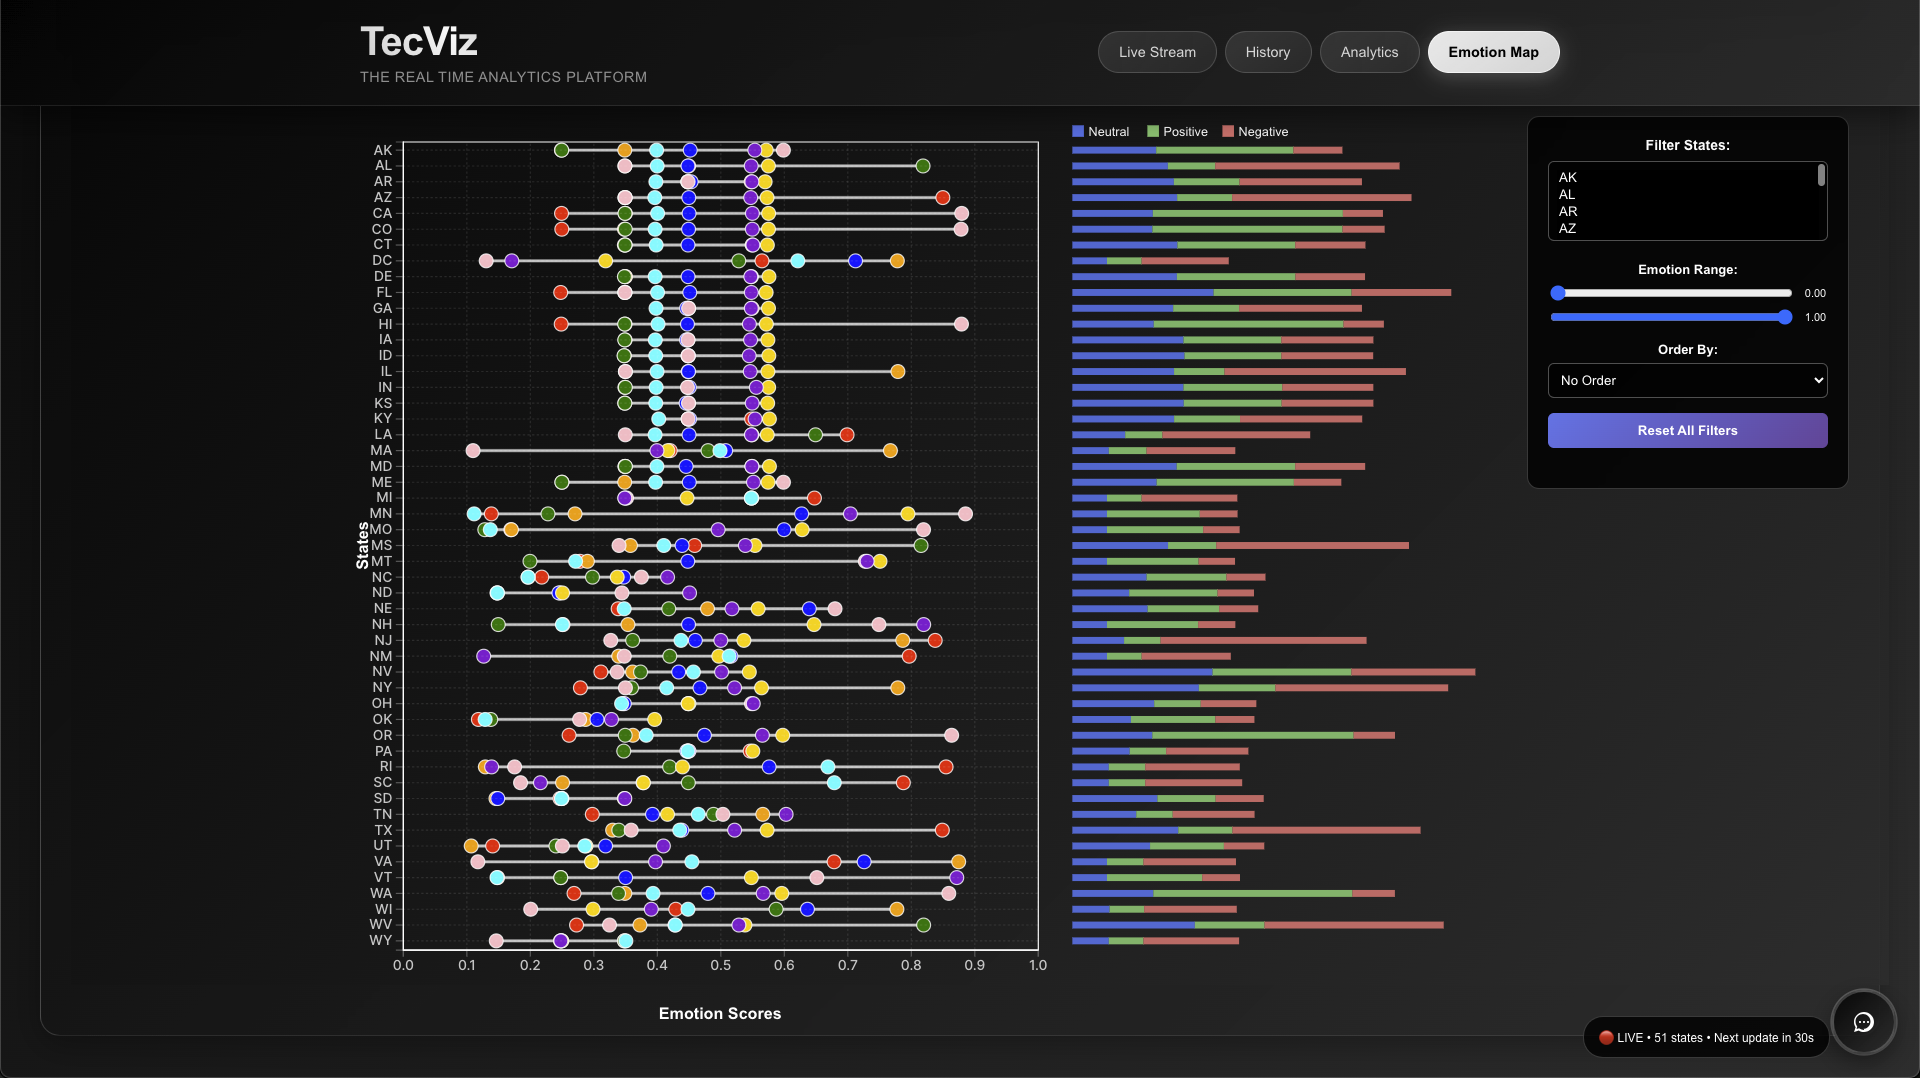
\includegraphics[width=0.95\textwidth]{Figures/Source/Emotion Dot Plot.png}
\caption{TECVis 1.0 Dot Plot: Multi-dimensional visualization showing emotion scores across all US states with interactive filters.}
\label{fig:landing_page}
\end{figure}

Each dot represents a state's average score for a specific emotion, enabling geographic comparison. Users can filter by emotion type and observe which states showed higher or lower scores for specific emotions. In TECVis 2.0, this visualization benefits from improved emotion detection accuracy (84\% vs. 41\%) while maintaining the same intuitive interface.

%----------------------------------------------------------------------------------------

\section{TECVis 2.0 Enhancements}

TECVis 2.0 extends the original system with new visualizations, real-time processing capabilities, and a conversational interface. This section demonstrates these enhancements.

\subsection{New Time Series Visualizations}

TECVis 2.0 introduces three new tabbed views for detailed time series analysis, accessible after clicking a state name from the main dashboard.

\subsubsection{Horizon Charts: Emotions Across a State}

Figure~\ref{fig:tab1_horizon} shows the first new visualization, displaying all emotions for a selected state over time using horizon charts.

\begin{figure}[htbp]
\centering
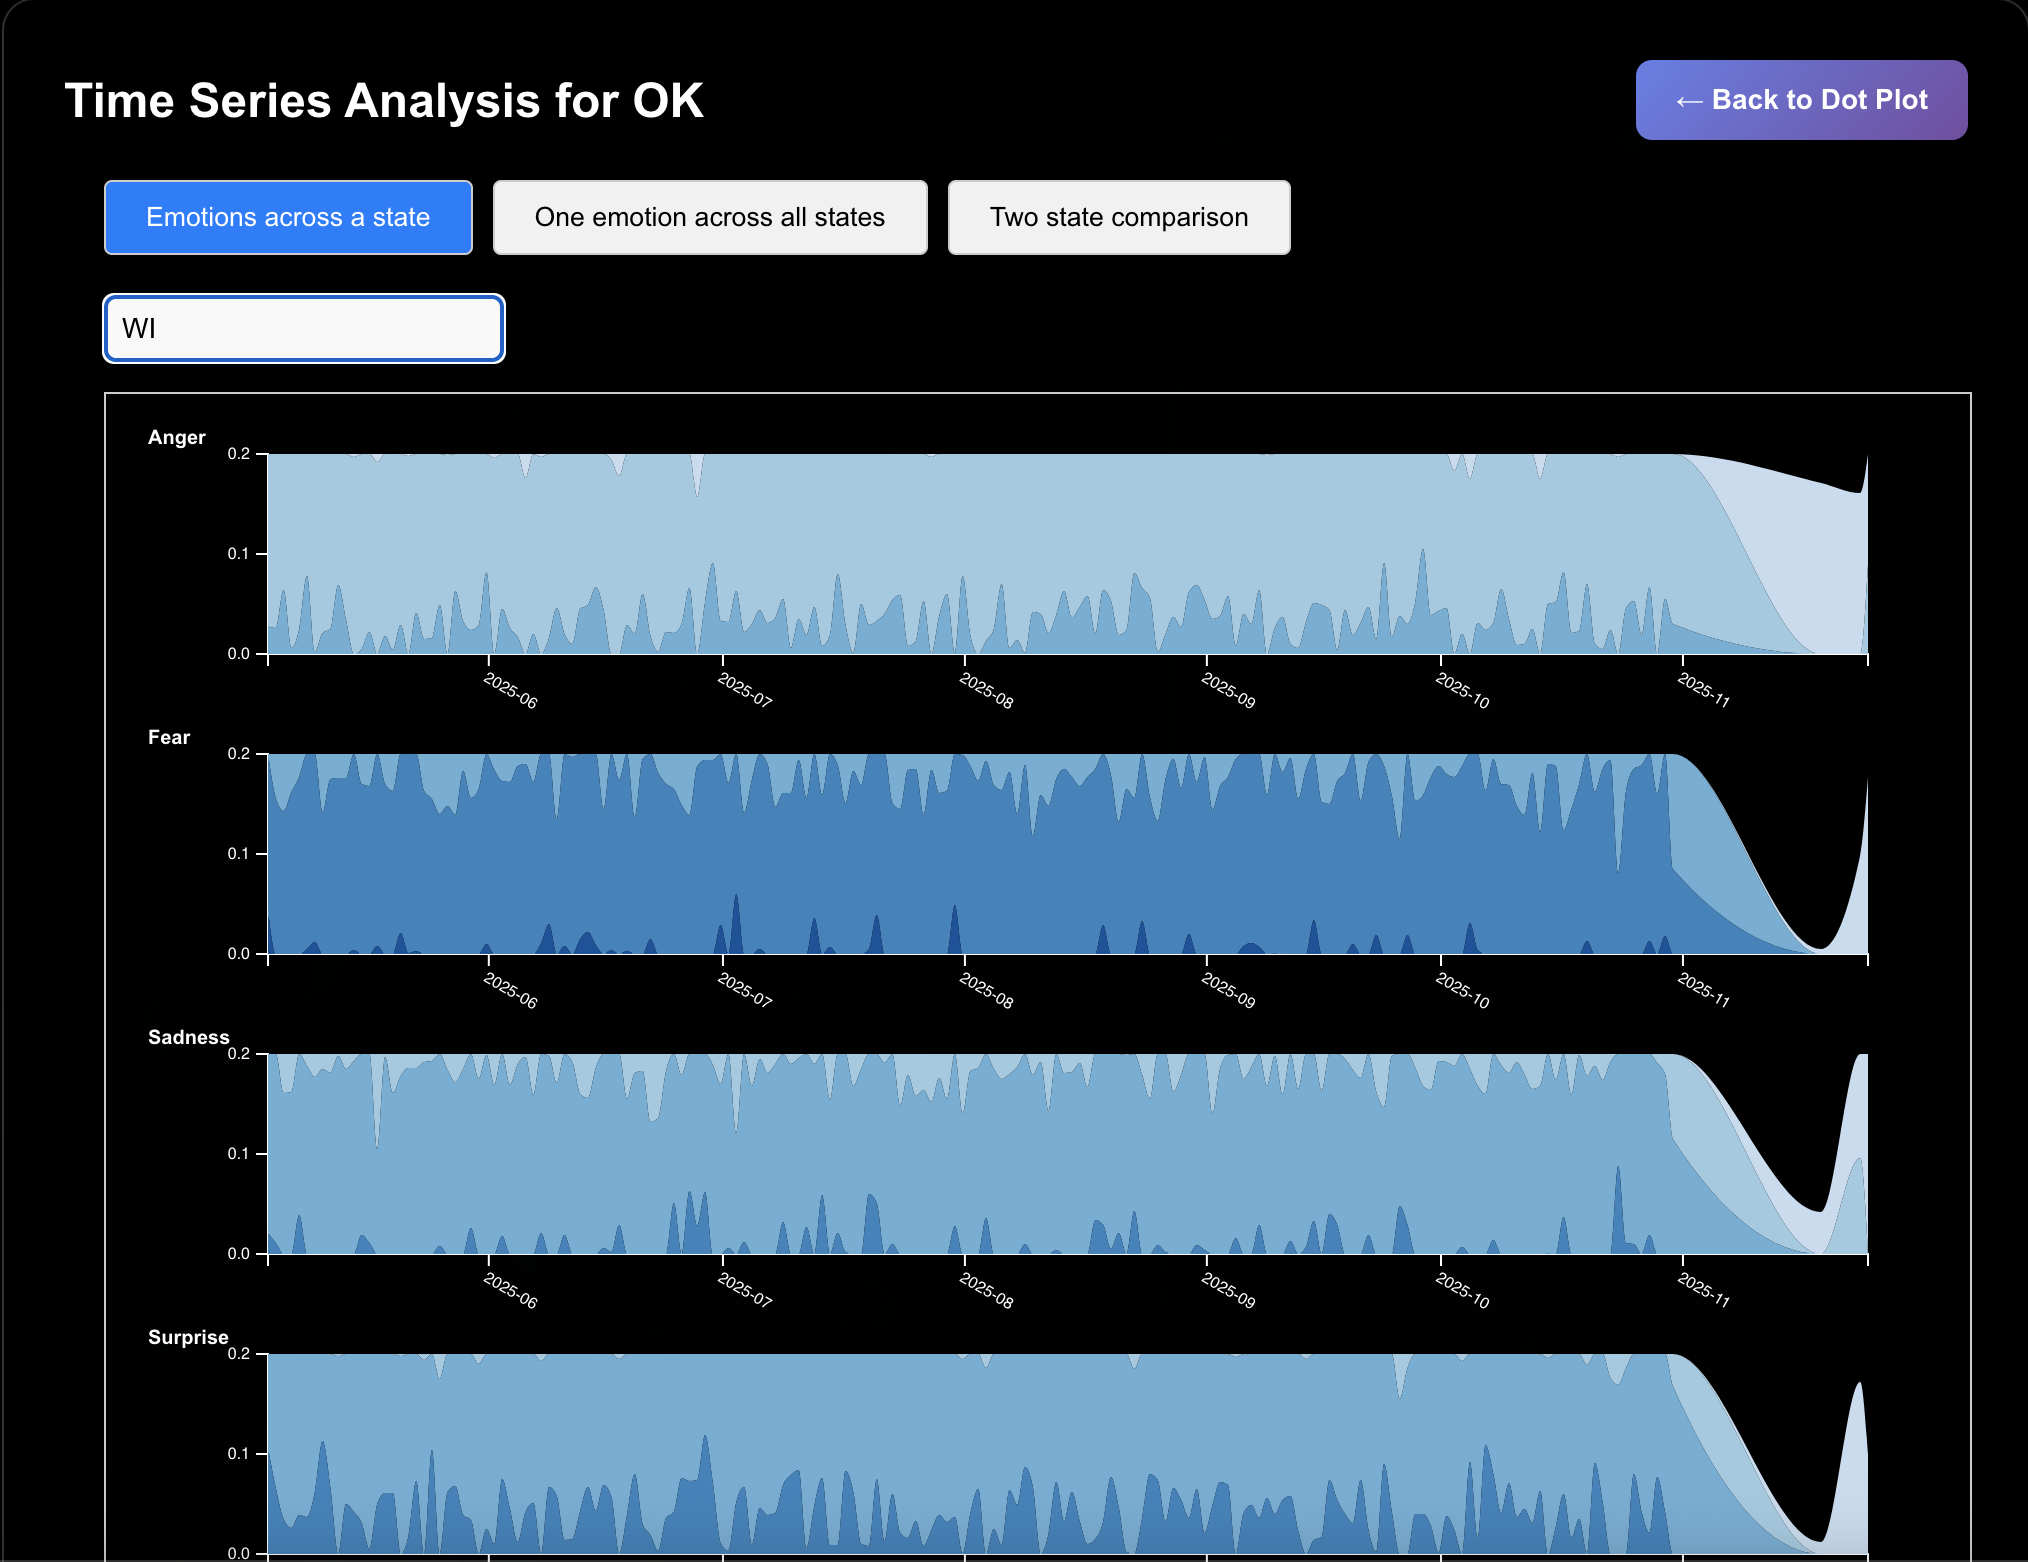
\includegraphics[width=0.85\textwidth]{Figures/Source/Emotion Across A State.png}
\caption{TECVis 2.0 Horizon Charts: All emotions for California over time with intensity bands.}
\label{fig:tab1_horizon}
\end{figure}

Horizon charts stack colored bands to show intensity without cluttering the display. Each emotion appears as a separate row, making it easy to spot peaks and trends. This visualization was not available in TECVis 1.0.

\subsubsection{Geographic Emotion Comparison}

Figure~\ref{fig:tab2_emotion_map} shows the second new visualization, displaying a single emotion across all states over time.

\begin{figure}[htbp]
\centering
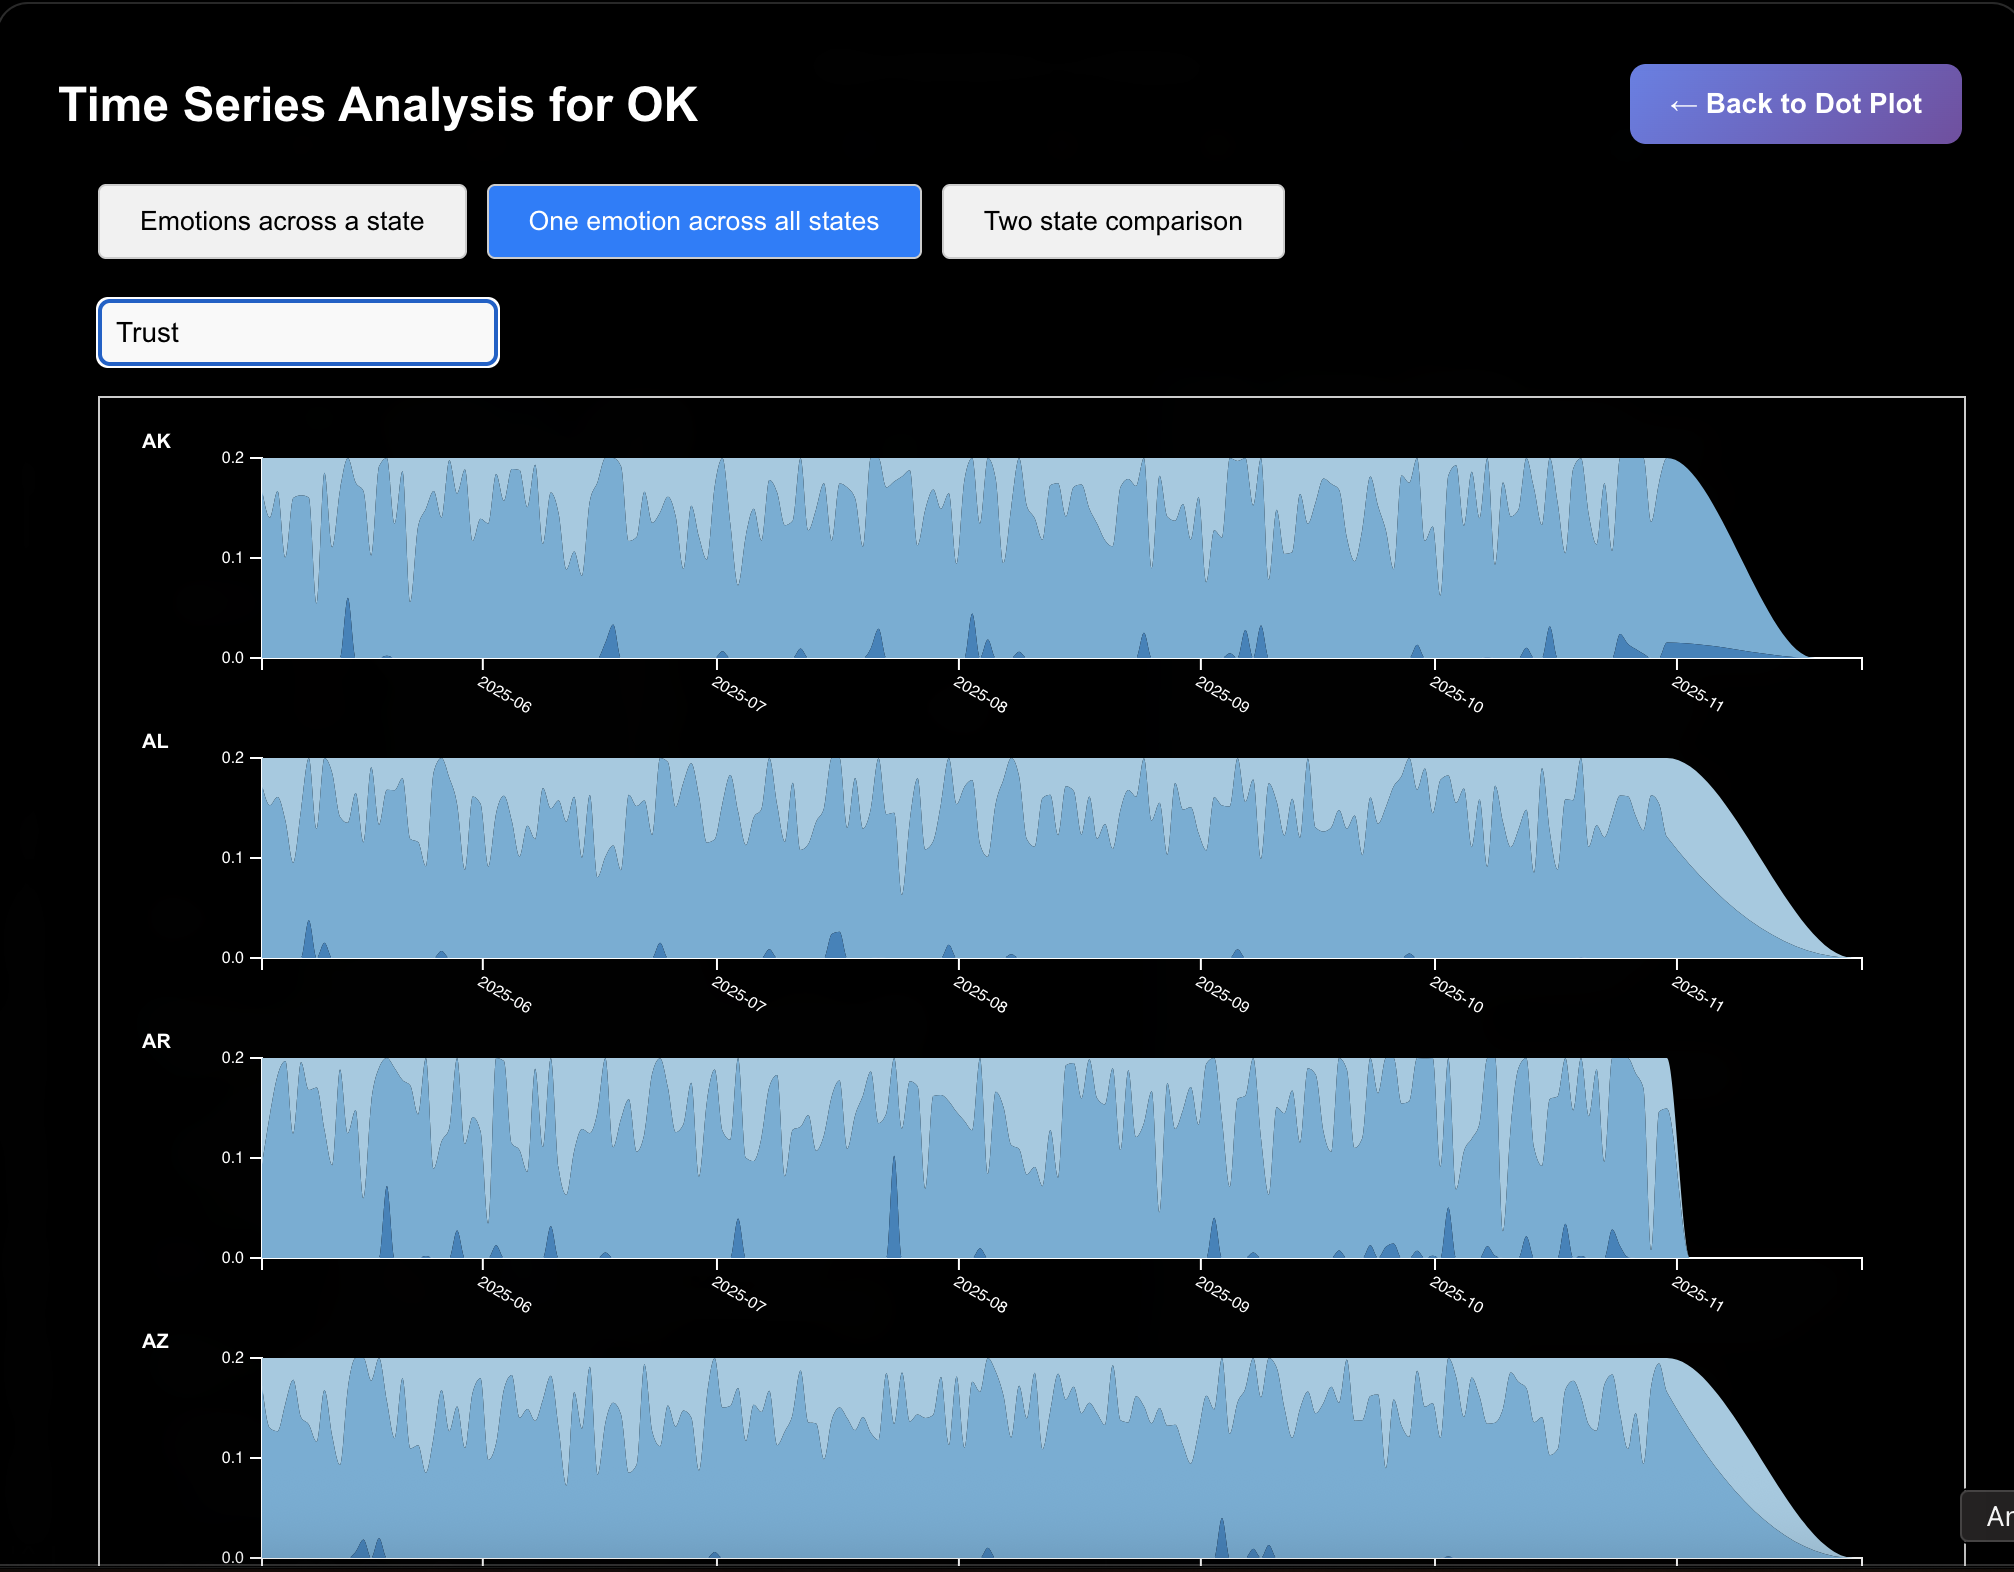
\includegraphics[width=0.85\textwidth]{Figures/Source/One emotion across all states.png}
\caption{TECVis 2.0 Geographic Comparison: Single emotion (fear) displayed across all states over time.}
\label{fig:tab2_emotion_map}
\end{figure}

This view enables geographic comparison of a single emotion, helping users identify which states experienced the highest or lowest levels of a specific emotion during a given period.

\subsubsection{Emotion Difference and Radar Charts}

Figures~\ref{fig:tab3_difference} and~\ref{fig:tab4_radar} show the emotion difference and radar visualizations, providing complementary comparison capabilities.

\begin{figure}[htbp]
\centering
\begin{subfigure}[b]{0.48\textwidth}
\centering
\includesvg[width=\textwidth]{Figures/Source/Emotion Difference}
\caption{Emotion Difference Chart: Comparing emotion levels between two states over time.}
\label{fig:tab3_difference}
\end{subfigure}
\hfill
\begin{subfigure}[b]{0.48\textwidth}
\centering
\includesvg[width=\textwidth]{Figures/Source/Emotion Radar}
\caption{Emotion Radar Chart: Multi-dimensional emotion profile comparison between two states.}
\label{fig:tab4_radar}
\end{subfigure}
\caption{TECVis 2.0 Comparison Visualizations: Difference chart (left) and radar chart (right) for state-level emotion analysis.}
\label{fig:comparison_charts}
\end{figure}

The difference chart visualizes where one state's emotion score exceeds the other, with positive and negative areas colored differently to enable precise comparison. The radar chart displays multiple emotions simultaneously, enabling users to compare emotional profiles between two states in a single view. Each axis represents a different emotion, making it easy to identify which states show similar or contrasting emotional patterns.
    
%----------------------------------------------------------------------------------------

\section{Real-Time Processing Implementation}

TECVis 2.0 implements a streaming architecture that processes data as it arrives, in contrast to TECVis 1.0's batch processing approach.

\subsection{Data Ingestion}

The tweet generation agent uses Ollama to generate realistic tweet text. The implementation configures Ollama with a prompt template, assigns state locations using weighted random distribution, timestamps each tweet, and publishes to Kafka using the kafka-python-ng library. The agent runs as a separate process, publishing tweets at configurable intervals (default: every 10 seconds).

The Kafka configuration includes the following parameters:

\begin{itemize}
\item \textbf{Replication factor:} Ensures data durability across multiple brokers
\item \textbf{Partition strategy:} Partitions tweets by state code for parallel processing
\item \textbf{Retention policy:} Retains messages for 7 days, enabling reprocessing
\item \textbf{Consumer groups:} Separate groups for raw data storage and NLP processing
\end{itemize}

\subsection{NLP Pipeline}

The NLP pipeline loads the following models:

\begin{itemize}
\item \textbf{DistilRoBERTa-Emotion:} Emotion classification head, returns probability distributions over seven emotions
\item \textbf{Twitter-RoBERTa:} Sentiment classification head, returns positive/negative/neutral labels
\item \textbf{GPU acceleration:} Models run on GPU when available, fallback to CPU otherwise
\end{itemize}

The preprocessing pipeline applies the following steps to tweet text:

\begin{itemize}
\item \textbf{URL removal:} Uses regex to identify and remove URLs
\item \textbf{Hashtag extraction:} Extracts words from hashtags, preserving semantic content
\item \textbf{Contraction expansion:} Uses dictionary to expand common contractions
\item \textbf{Character normalization:} Reduces repeated characters to maximum of two repetitions
\item \textbf{Text cleaning:} Removes special characters that don't contribute to emotion detection
\end{itemize}

\subsection{Database and API}

The PostgreSQL database schema includes the following components:

\begin{itemize}
\item \textbf{Raw tweets table:} Stores original tweet text, timestamp, location, and metadata
\item \textbf{Processed tweets table:} Stores emotion scores, sentiment labels, and confidence scores
\item \textbf{Aggregation tables:} Pre-computed state-level and time-based aggregations for fast queries
\item \textbf{Indexes:} Optimized indexes on timestamp, state\_code, and dominant\_emotion
\end{itemize}

Table~\ref{tab:api_endpoints} lists the REST API endpoints.

\begin{table}[htbp]
\centering
\caption{REST API Endpoints}
\label{tab:api_endpoints}
\begin{tabular}{lp{8cm}}
\hline
\textbf{Endpoint} & \textbf{Function} \\
\hline
GET /api/dashboard & Returns aggregated emotion scores for the main dashboard \\
GET /api/timeseries & Returns time series data for specific states or emotions \\
GET /api/comparison & Returns comparison data for two states \\
GET /api/states & Returns list of available states \\
GET /api/emotions & Returns list of available emotions \\
\hline
\end{tabular}
\end{table}

The API uses Server-Sent Events (SSE) to stream new data as it arrives, maintaining persistent connections with clients and sending updates when new tweets are processed.

%----------------------------------------------------------------------------------------

\section{Conversational Interface}

TECVis 2.0 introduces a conversational chatbot interface that was not available in TECVis 1.0. This feature enables users to query emotion data using natural language.

Figure~\ref{fig:chatbot_flow} shows the complete chatbot system flow, from user query to visualization.

\begin{figure}[htbp]
\centering
\includesvg[width=0.95\textwidth]{Figures/Source/chatbot_flow}
\caption{Chatbot System Flow: Complete pipeline from natural language query to SQL translation, query execution, chart selection, and response generation.}
\label{fig:chatbot_flow}
\end{figure}

\subsection{Query Interface}

The chatbot interface enables users to ask questions in plain English, without requiring knowledge of SQL or database schemas. Figure~\ref{fig:chatbot_query} shows an example query asking about emotion trends.

\begin{figure}[htbp]
\centering
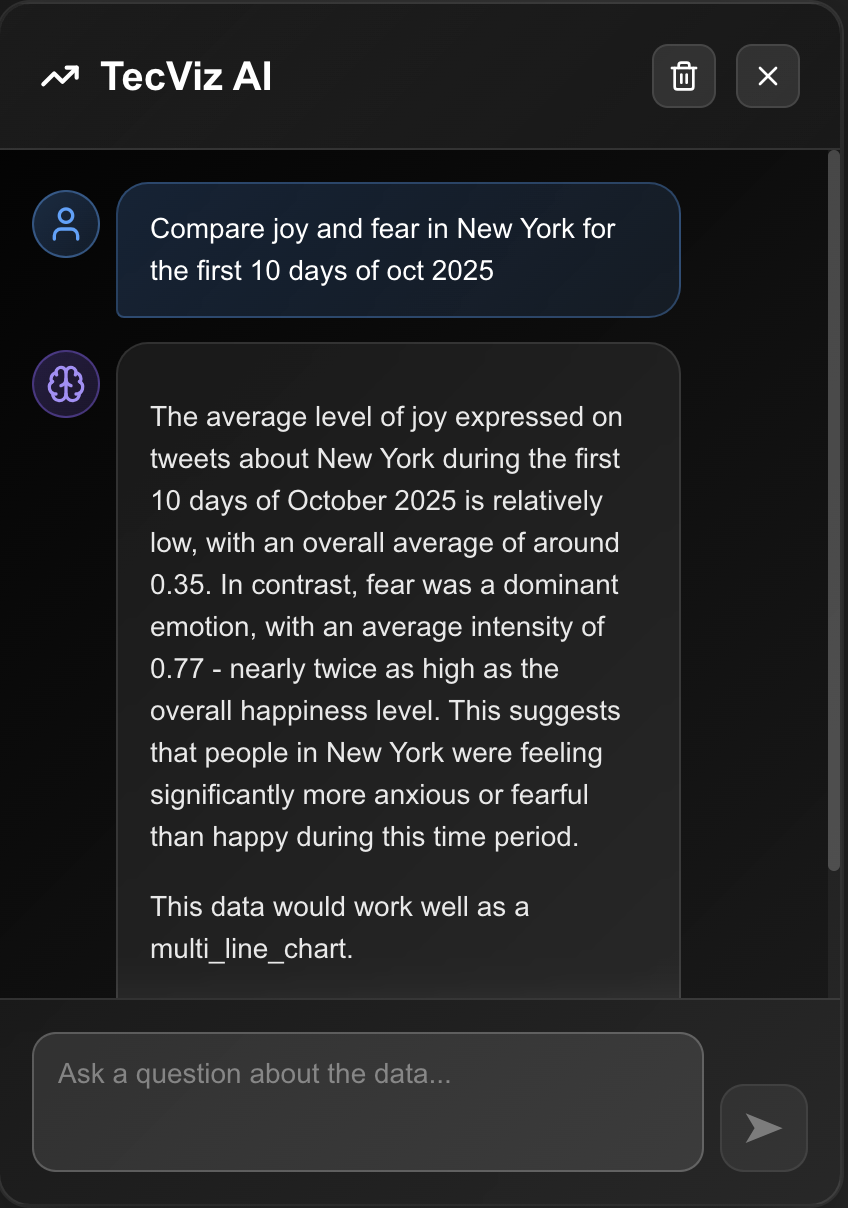
\includegraphics[width=0.85\textwidth]{Figures/Source/Chatbot.png}
\caption{Chatbot Query Interface: Example query asking about emotion trends across states.}
\label{fig:chatbot_query}
\end{figure}

After query execution, the chatbot presents results through an interactive modal that provides transparency into the system's reasoning. Figure~\ref{fig:chatbot_modal} shows the result modal with its three-tab interface.

\begin{figure}[htbp]
\centering
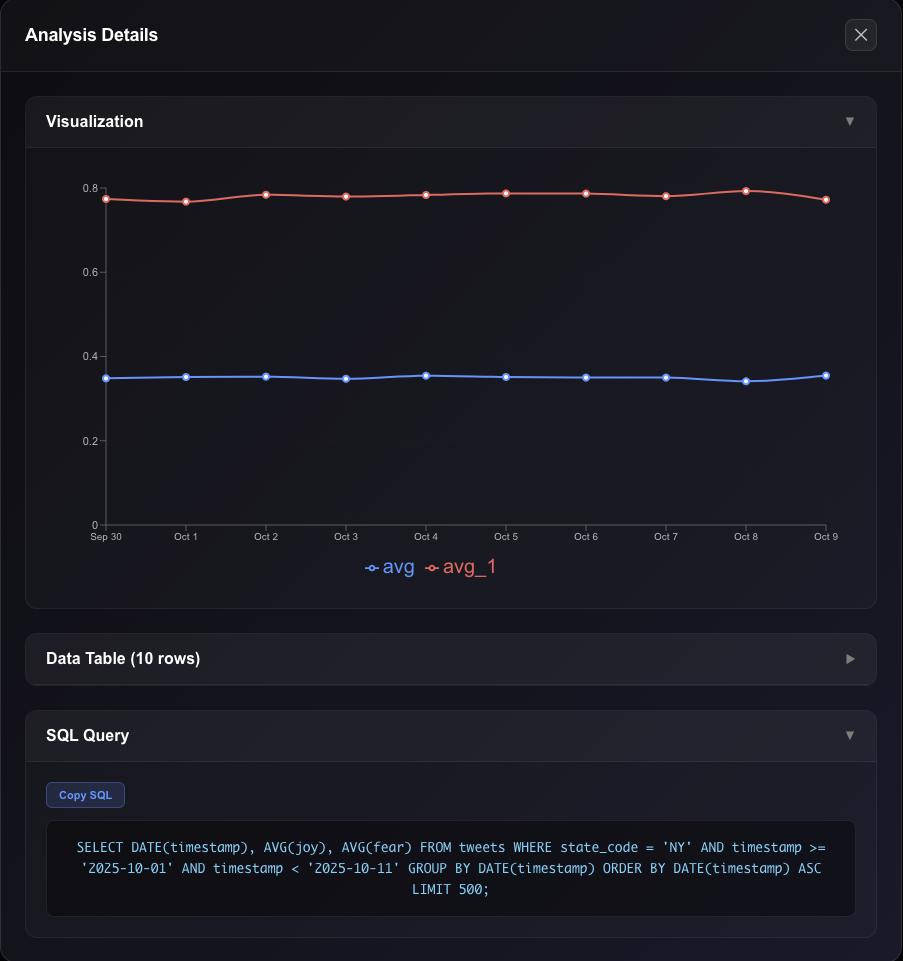
\includegraphics[width=0.85\textwidth]{Figures/Source/Chatbot Result.png}
\caption{Chatbot Result Modal: Three-tab interface showing SQL query, raw data, and visualization.}
\label{fig:chatbot_modal}
\end{figure}

The chatbot uses Ollama (Mistral model) for NL2SQL translation, validates generated SQL before execution, executes queries against PostgreSQL, analyzes results to select appropriate chart type, and generates natural language summaries. The modal provides transparency through three tabs: SQL (shows generated query), Data (displays raw results), and Visualization (renders selected chart). This design enables users to understand how their natural language question was interpreted and what data was retrieved.

\subsection{Query and Result Variability}

The chatbot handles diverse query types, from simple aggregations to complex multi-state comparisons. Figure~\ref{fig:chatbot_query2} demonstrates another query example, showing how the system adapts to different question formats and intents.

\begin{figure}[htbp]
\centering
\includesvg[width=0.85\textwidth]{Figures/Source/Chatbot2}
\caption{Chatbot Query Variability: Different query types demonstrating the system's adaptability to various question formats.}
\label{fig:chatbot_query2}
\end{figure}

Figure~\ref{fig:chatbot_result2} demonstrates another result example, showing how the system adapts visualizations based on query results. Different query types produce different chart types, with the system automatically selecting the most appropriate visualization for the data structure and user intent.

\begin{figure}[htbp]
    \centering
\includesvg[width=0.85\textwidth]{Figures/Source/Chatbot Result}
\caption{Chatbot Result Variability: Different result visualizations demonstrating adaptive chart selection based on query results.}
\label{fig:chatbot_result2}
    \end{figure}

\subsection{Chart Selection}

The chart suggestion agent selects visualization types based on query intent:

\begin{itemize}
\item \textbf{Stacked bar charts:} Composition queries (breakdowns, percentages)
\item \textbf{Line charts:} Time series queries (trends over time)
\item \textbf{Radar charts:} Multi-dimensional profile comparisons
\item \textbf{Grouped bar charts:} Side-by-side metric comparisons
\item \textbf{Tornado charts:} Two-state comparisons
\end{itemize}

%----------------------------------------------------------------------------------------

\section{Summary}

This chapter has demonstrated the system through a narrative progression: first showing the visualizations inherited from TECVis 1.0 (dot plot), then presenting the new enhancements in TECVis 2.0 (horizon charts, difference charts, radar charts, real-time processing, and conversational interface). The implementation follows the architecture described in Chapter 4, with modular components that can be developed, tested, and deployed independently. The next chapter evaluates the system's performance and user experience.

%----------------------------------------------------------------------------------------
